%!TEX encoding = UTF-8
\documentclass[uplatex]{jsarticle}
\usepackage[dvipdfmx]{graphicx, color}
\usepackage{bmpsize}
\usepackage{wrapfig}
\usepackage{url}

\title{情報特論}
\author{32番 松川侑生}
\date{\today}

\begin{document}
\maketitle
\section{目的}
    Tello EDUの単眼カメラとDlibの顔検出を利用して顔追跡をおこなう。
\section{開発環境}
    \textit{Tello EDUの公式サイト}~\cite{tello}より、本体情報をに示す。

    ノートパソコン\\
\section{設計仕様}
    \begin{wrapfigure}{r}{0.5\textwidth}
        \begin{center}
        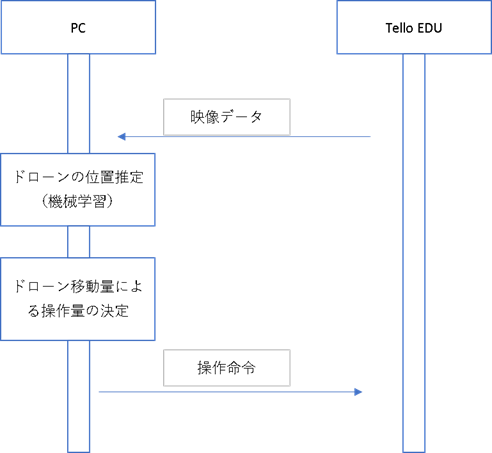
\includegraphics[width=0.5\textwidth]{sequence.png}
        \end{center}
        \caption{sequence}
    \end{wrapfigure}
    
\section{開発結果}
\section{考察}
asdfg a
fasdg

\textit{Molecular Cell Biology}~\cite{mcbe} (日本語訳は「分子細胞生物学」~\cite{mcb})は
\textit{Molecular Biology of the Cell}と並んで、しばしば分子生物学の
入門書として読まれる本です。

\bibliographystyle{jplain}
\bibliography{refer}

\end{document}